\documentclass{article}
\usepackage{graphicx}
\usepackage{tikz}
\usepackage{enumitem}
\usepackage{amssymb}
\usepackage{amsmath}
\usepackage{xcolor}
\usepackage{color, colortbl}
\newcommand*{\defeq}{\stackrel{\text{def}}{=}}
\title{Tugas Aljabar I}
\author{Teosofi Hidayah Agung\\
5002221132}
\date{}
\begin{document}
\maketitle
\pagenumbering{gobble}
\setlength{\belowdisplayskip}{-4.5mm}
\setlength{\abovedisplayskip}{1.5mm}
\allowdisplaybreaks

    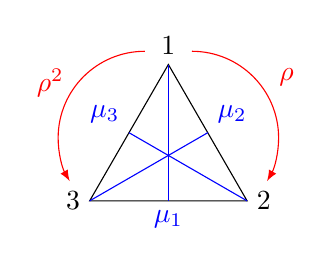
\begin{tikzpicture}
        \coordinate[label=above:1] (A) at (3,1.732050807568877);
        \coordinate[label=right:2] (B) at (4,0);
        \coordinate[label=left:3] (C) at (2,0);
        \coordinate[label=below:$\color{blue}\mu_1$] (M1) at (3,0);
        \coordinate[label=above right:$\color{blue}\mu_2$] (M2) at (3.5,0.866025);
        \coordinate[label=above left:$\color{blue}\mu_3$] (M3) at (2.5,0.866025);

        
        \draw (C)--(A)--(B)--cycle;
        \draw[blue] (A)--(M1);
        \draw[blue] (C)--(M2);
        \draw[blue] (B)--(M3);

        \draw[-latex,red] (3.3,1.9) arc
            [
            start angle=90,
            end angle=-30,
            x radius=1.1cm,
            y radius =1.1cm
            ] ;
        \coordinate[label=below:$\color{red}\rho$] (R1) at (4.5,1.8);
        \coordinate[label=below:$\color{red}\rho^2$] (R1) at (1.5,1.8);
        \draw[-latex,red] (2.7,1.9) arc
            [
            start angle=90,
            end angle=210,
            x radius=1.1cm,
            y radius =1.1cm
            ] ;
    \end{tikzpicture}
    \begin{flalign*}
        \rho_0&=\begin{pmatrix}1\end{pmatrix}&\\
        \rho&=\begin{pmatrix}1&2&3\end{pmatrix}&\\
        \rho^2&=\begin{pmatrix}1&3&2\end{pmatrix}&\\
        \mu_1&=\begin{pmatrix}2&3\end{pmatrix}&\\
        \mu_2&=\begin{pmatrix}1&2\end{pmatrix}&\\
        \mu_3&=\begin{pmatrix}1&3\end{pmatrix}&\\
        D_3&=\{\rho_0,\rho_1,\rho_2,\mu_1,\mu_2,\mu_3\}&\\
    \end{flalign*}\\
    Komposisi:
    \begin{itemize}
        \item $\rho_0\circ\rho_0 =\begin{pmatrix}1\end{pmatrix}\circ\begin{pmatrix}1\end{pmatrix}=\begin{pmatrix}1\end{pmatrix}=\rho_0$
        \item $\rho_0\circ\rho =\begin{pmatrix}1\end{pmatrix}\circ\begin{pmatrix}1&2&3\end{pmatrix}=\begin{pmatrix}1&2&3\end{pmatrix}=\rho$
        \item $\rho_0\circ\rho^2 =\begin{pmatrix}1\end{pmatrix}\circ\begin{pmatrix}1&3&2\end{pmatrix}=\begin{pmatrix}1&3&2\end{pmatrix}=\rho^2$
        \item $\rho_0\circ\mu_1 =\begin{pmatrix}1\end{pmatrix}\circ\begin{pmatrix}2&3\end{pmatrix}=\begin{pmatrix}2&3\end{pmatrix}=\mu_1$
        \item $\rho_0\circ\mu_2 =\begin{pmatrix}1\end{pmatrix}\circ\begin{pmatrix}1&2\end{pmatrix}=\begin{pmatrix}1&2\end{pmatrix}=\mu_2$
        \item $\rho_0\circ\mu_3 =\begin{pmatrix}1\end{pmatrix}\circ\begin{pmatrix}1&3\end{pmatrix}=\begin{pmatrix}1&3\end{pmatrix}=\mu_1$
        
        \item $\rho\circ\rho_0 =\begin{pmatrix}1&2&3\end{pmatrix}\circ\begin{pmatrix}1\end{pmatrix}=\begin{pmatrix}1&2&3\end{pmatrix}=\rho$
        \item $\rho\circ\rho =\begin{pmatrix}1&2&3\end{pmatrix}\circ\begin{pmatrix}1&2&3\end{pmatrix}=\begin{pmatrix}1&3&2\end{pmatrix}=\rho^2$
        \item $\rho\circ\rho^2 =\begin{pmatrix}1&2&3\end{pmatrix}\circ\begin{pmatrix}1&3&2\end{pmatrix}=\begin{pmatrix}1\end{pmatrix}=\rho_0$
        \item $\rho\circ\mu_1 =\begin{pmatrix}1&2&3\end{pmatrix}\circ\begin{pmatrix}2&3\end{pmatrix}=\begin{pmatrix}1&2\end{pmatrix}=\mu_2$
        \item $\rho\circ\mu_2 =\begin{pmatrix}1&2&3\end{pmatrix}\circ\begin{pmatrix}1&2\end{pmatrix}=\begin{pmatrix}1&3\end{pmatrix}=\mu_3$
        \item $\rho\circ\mu_3 =\begin{pmatrix}1&2&3\end{pmatrix}\circ\begin{pmatrix}1&3\end{pmatrix}=\begin{pmatrix}2&3\end{pmatrix}=\mu_1$

        \item $\rho^2\circ\rho_0 =\begin{pmatrix}1&3&2\end{pmatrix}\circ\begin{pmatrix}1\end{pmatrix}=\begin{pmatrix}1&3&2\end{pmatrix}=\rho^2$
        \item $\rho^2\circ\rho =\begin{pmatrix}1&3&2\end{pmatrix}\circ\begin{pmatrix}1&2&3\end{pmatrix}=\begin{pmatrix}1\end{pmatrix}=\rho_0$
        \item $\rho^2\circ\rho^2 =\begin{pmatrix}1&3&2\end{pmatrix}\circ\begin{pmatrix}1&3&2\end{pmatrix}=\begin{pmatrix}1&2&3\end{pmatrix}=\rho$
        \item $\rho^2\circ\mu_1 =\begin{pmatrix}1&3&2\end{pmatrix}\circ\begin{pmatrix}2&3\end{pmatrix}=\begin{pmatrix}1&3\end{pmatrix}=\mu_3$
        \item $\rho^2\circ\mu_2 =\begin{pmatrix}1&3&2\end{pmatrix}\circ\begin{pmatrix}1&2\end{pmatrix}=\begin{pmatrix}2&3\end{pmatrix}=\mu_1$
        \item $\rho^2\circ\mu_1 =\begin{pmatrix}1&3&2\end{pmatrix}\circ\begin{pmatrix}1&3\end{pmatrix}=\begin{pmatrix}1&2\end{pmatrix}=\mu_2$
        
        \item $\mu_1\circ\rho_0 =\begin{pmatrix}2&3\end{pmatrix}\circ\begin{pmatrix}1\end{pmatrix}=\begin{pmatrix}2&3\end{pmatrix}=\mu_1$
        \item $\mu_1\circ\rho =\begin{pmatrix}2&3\end{pmatrix}\circ\begin{pmatrix}1&2&3\end{pmatrix}=\begin{pmatrix}2&3\end{pmatrix}=\mu_3$
        \item $\mu_1\circ\rho^2 =\begin{pmatrix}2&3\end{pmatrix}\circ\begin{pmatrix}1&3&2\end{pmatrix}=\begin{pmatrix}1&2\end{pmatrix}=\mu_2$
        \item $\mu_1\circ\mu_1 =\begin{pmatrix}2&3\end{pmatrix}\circ\begin{pmatrix}2&3\end{pmatrix}=\begin{pmatrix}1\end{pmatrix}=\rho_0$
        \item $\mu_1\circ\mu_2 =\begin{pmatrix}2&3\end{pmatrix}\circ\begin{pmatrix}1&2\end{pmatrix}=\begin{pmatrix}1&3&2\end{pmatrix}=\rho^2$
        \item $\mu_1\circ\mu_3 =\begin{pmatrix}2&3\end{pmatrix}\circ\begin{pmatrix}1&3\end{pmatrix}=\begin{pmatrix}1&2&3\end{pmatrix}=\rho$

        \item $\mu_2\circ\rho_0 =\begin{pmatrix}1&2\end{pmatrix}\circ\begin{pmatrix}1\end{pmatrix}=\begin{pmatrix}1&2\end{pmatrix}=\mu_2$
        \item $\mu_2\circ\rho =\begin{pmatrix}1&2\end{pmatrix}\circ\begin{pmatrix}1&2&3\end{pmatrix}=\begin{pmatrix}2&3\end{pmatrix}=\mu_1$
        \item $\mu_2\circ\rho^2 =\begin{pmatrix}1&2\end{pmatrix}\circ\begin{pmatrix}1&3&2\end{pmatrix}=\begin{pmatrix}1&3\end{pmatrix}=\mu_3$
        \item $\mu_2\circ\mu_1 =\begin{pmatrix}1&2\end{pmatrix}\circ\begin{pmatrix}2&3\end{pmatrix}=\begin{pmatrix}1&2&3\end{pmatrix}=\rho$
        \item $\mu_2\circ\mu_2 =\begin{pmatrix}1&2\end{pmatrix}\circ\begin{pmatrix}1&2\end{pmatrix}=\begin{pmatrix}1\end{pmatrix}=\rho_0$
        \item $\mu_2\circ\mu_3 =\begin{pmatrix}1&2\end{pmatrix}\circ\begin{pmatrix}1&3\end{pmatrix}=\begin{pmatrix}1&3&2\end{pmatrix}=\rho^2$
        
        \item $\mu_3\circ\rho_0 =\begin{pmatrix}1&3\end{pmatrix}\circ\begin{pmatrix}1\end{pmatrix}=\begin{pmatrix}1&3\end{pmatrix}=\mu_3$
        \item $\mu_3\circ\rho =\begin{pmatrix}1&3\end{pmatrix}\circ\begin{pmatrix}1&2&3\end{pmatrix}=\begin{pmatrix}1&2\end{pmatrix}=\mu_2$
        \item $\mu_3\circ\rho^2 =\begin{pmatrix}1&3\end{pmatrix}\circ\begin{pmatrix}1&3&2\end{pmatrix}=\begin{pmatrix}2&3\end{pmatrix}=\mu_1$
        \item $\mu_3\circ\mu_1 =\begin{pmatrix}1&3\end{pmatrix}\circ\begin{pmatrix}2&3\end{pmatrix}=\begin{pmatrix}1&3&2\end{pmatrix}=\rho^2$
        \item $\mu_3\circ\mu_2 =\begin{pmatrix}1&3\end{pmatrix}\circ\begin{pmatrix}1&2\end{pmatrix}=\begin{pmatrix}1&2&3\end{pmatrix}=\rho$
        \item $\mu_3\circ\mu_3 =\begin{pmatrix}1&3\end{pmatrix}\circ\begin{pmatrix}1&3\end{pmatrix}=\begin{pmatrix}1\end{pmatrix}=\rho_0$
    \end{itemize}
    \newcolumntype{l}{>{\columncolor{lime}}c}
    \begin{center}
    \begin{tabular}{|l|| c c c c c c|} 
        \hline
        \rowcolor{cyan}
         \color{purple}$\circ$ & $\rho_0$ & $\rho$ & $\rho^2$ & $\mu_1$ & $\mu_2$ & $\mu_3$\\
         \hline\hline
         $\rho_0$ & $\rho_0$ & $\rho$ & $\rho^2$ & $\mu_1$ & $\mu_2$ & $\mu_3$\\
         $\rho$ & $\rho$ & $\rho^2$ & $\rho_0$ & $\mu_2$ & $\mu_3$ & $\mu_1$\\
         $\rho^2$ & $\rho^2$ & $\rho_0$ & $\rho$ & $\mu_3$ & $\mu_1$ & $\mu_2$\\
         $\mu_1$ & $\mu_1$ & $\mu_3$ & $\mu_2$ & $\rho_0$ & $\rho^2$ & $\rho$\\
         $\mu_2$ & $\mu_2$ & $\mu_1$ & $\mu_3$ & $\rho$ & $\rho_0$ & $\rho^2$\\
         $\mu_3$ & $\mu_3$ & $\mu_2$ & $\mu_1$ & $\rho^2$ & $\rho$ & $\rho_0$\\
         \hline
    \end{tabular}
    
    \vspace{0.9mm}
    Tabel komposisi
    \end{center}
    
    \begin{center}
    \line(1,0){340}
    \end{center}

    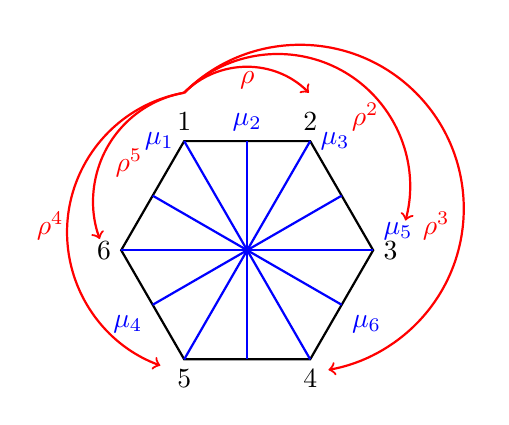
\begin{tikzpicture}[thick, scale=0.4]
        \coordinate[label=above:1] (A) at (-2,3.464101615137755);
        \coordinate[label=above:2] (B) at (2,3.464101615137755);
        \coordinate[label=right:3] (C) at (4,0);
        \coordinate[label=below:4] (D) at (2,-3.464101615137755);
        \coordinate[label=below:5] (E) at (-2,-3.464101615137755);
        \coordinate[label=left:6] (F) at (-4,0);
        \coordinate[label=left:$\color{blue}\mu_1$] (M1) at (A);
        \coordinate[label=above:$\color{blue}\mu_2$] (M2) at (0,3.464101615137755);
        \coordinate[label=right:$\color{blue}\mu_3$] (M3) at (B);
        \coordinate[label=below left:$\color{blue}\mu_4$] (M4) at (-3,-1.732050807568877);
        \coordinate[label=above right:$\color{blue}\mu_5$] (M5) at (C);
        \coordinate[label=below right:$\color{blue}\mu_6$] (M6) at (3,-1.732050807568877);
        \coordinate[label=below:$\color{red}\rho$] (R1) at (0,6);
        \coordinate[label=below left:$\color{red}\rho^2$] (R2) at (4.5,5);
        \coordinate[label=above:$\color{red}\rho^3$] (R3) at (6,0);
        \coordinate[label=above left:$\color{red}\rho^4$] (R4) at (-5.5,0);
        \coordinate[label=above left:$\color{red}\rho^5$] (R5) at (-3,2);

        \draw (A)--(B)--(C)--(D)--(E)--(F)--cycle;
        \draw[blue] (A)--(D);
        \draw[blue] (M2)--(0,-3.464101615137755);
        \draw[blue] (B)--(E);
        \draw[blue] (M4)--(3,1.732050807568877);
        \draw[blue] (C)--(F);
        \draw[blue] (M6)--(-3,1.732050807568877);

        \draw[thick, ->,red] (-2,5) arc (135:45:2.8);
        \draw[thick, ->,red] (-2,5) arc (135:-15:4.2);
        \draw[thick, ->,red] (-2,5) arc (135:-80:5.2);
        \draw[thick, ->,red] (-2,5) arc (100:250:4.5);
        \draw[thick, ->,red] (-2,5) arc (100:200:3.5);
    \end{tikzpicture}
\begin{enumerate}

    \item Tentukan anggota $D_6$?\\~\\
    \textbf{Jawab}:
        \begin{itemize}
            \item $\rho_0=\begin{pmatrix}1\end{pmatrix}$
            \item $\rho=\begin{pmatrix}1&2&3&4&5&6\end{pmatrix}$
            \item $\rho^2=\begin{pmatrix}1&3&5\end{pmatrix}\begin{pmatrix}2&4&6\end{pmatrix}$
            \item $\rho^3=\begin{pmatrix}1&4\end{pmatrix}\begin{pmatrix}2&5\end{pmatrix}\begin{pmatrix}3&6\end{pmatrix}$
            \item $\rho^4=\begin{pmatrix}1&5&3\end{pmatrix}\begin{pmatrix}2&6&4\end{pmatrix}$
            \item $\rho^5=\begin{pmatrix}6&5&4&3&2&1\end{pmatrix}$
            \item $\mu_1=\begin{pmatrix}2&6\end{pmatrix}\begin{pmatrix}3&5\end{pmatrix}$
            \item $\mu_2=\begin{pmatrix}1&2\end{pmatrix}\begin{pmatrix}3&6\end{pmatrix}\begin{pmatrix}4&5\end{pmatrix}$
            \item $\mu_3=\begin{pmatrix}1&3\end{pmatrix}\begin{pmatrix}4&6\end{pmatrix}$
            \item $\mu_4=\begin{pmatrix}2&3\end{pmatrix}\begin{pmatrix}1&4\end{pmatrix}\begin{pmatrix}5&6\end{pmatrix}$
            \item $\mu_5=\begin{pmatrix}1&5\end{pmatrix}\begin{pmatrix}2&4\end{pmatrix}$
            \item $\mu_6=\begin{pmatrix}3&4\end{pmatrix}\begin{pmatrix}2&5\end{pmatrix}\begin{pmatrix}1&6\end{pmatrix}$
        \end{itemize}
        
    \item Tunjukkan bahwa\\~\\
    \textbf{Jawab}:
        \begin{flalign*}
            %mu 2
            \bullet \rho\circ\mu_1 &=\begin{pmatrix}1&2&3&4&5&6\end{pmatrix}\circ\begin{pmatrix}2&6\end{pmatrix}\begin{pmatrix}3&5\end{pmatrix}&\\
            &=\begin{pmatrix}1&2\end{pmatrix}\begin{pmatrix}3&6\end{pmatrix}\begin{pmatrix}4&5\end{pmatrix}=\mu_2&\\
            %mu 3
            \bullet \rho^2\circ\mu_1 &=\begin{pmatrix}1&3&5\end{pmatrix}\begin{pmatrix}2&4&6\end{pmatrix} \circ\begin{pmatrix}2&6\end{pmatrix}\begin{pmatrix}3&5\end{pmatrix}&\\
            &=\begin{pmatrix}1&3\end{pmatrix}\begin{pmatrix}4&6\end{pmatrix}=\mu_3&\\
            %mu 4
            \bullet \rho^3\circ\mu_1 &=\begin{pmatrix}1&4\end{pmatrix}\begin{pmatrix}2&5\end{pmatrix}\begin{pmatrix}3&6\end{pmatrix} \circ\begin{pmatrix}2&6\end{pmatrix}\begin{pmatrix}3&5\end{pmatrix}&\\
            &=\begin{pmatrix}2&3\end{pmatrix}\begin{pmatrix}1&4\end{pmatrix}\begin{pmatrix}5&6\end{pmatrix}=\mu_4&\\
            %mu 5
            \bullet \rho^4\circ\mu_1 &=\begin{pmatrix}1&5&3\end{pmatrix}\begin{pmatrix}2&6&4\end{pmatrix} \circ\begin{pmatrix}2&6\end{pmatrix}\begin{pmatrix}3&5\end{pmatrix}&\\
            &=\begin{pmatrix}1&5\end{pmatrix}\begin{pmatrix}2&4\end{pmatrix}=\mu_5&\\
            %mu 6
            \bullet \rho^5\circ\mu_1 &=\begin{pmatrix}6&5&4&3&2&1\end{pmatrix}\circ\begin{pmatrix}2&6\end{pmatrix}\begin{pmatrix}3&5\end{pmatrix}&\\
            &=\begin{pmatrix}3&4\end{pmatrix}\begin{pmatrix}2&5\end{pmatrix}\begin{pmatrix}1&6\end{pmatrix}=\mu_6&\\
        \end{flalign*}
        
    \item Tentukan $k$ sehingga $\rho^2\mu_1=\mu_1\rho^k$.\\~\\
    \textbf{Jawab}:\\
    Dengan sebuah teorema maka didapat $k=4$, buktinya:
    \begin{flalign*}
        \rho^2\mu_1&=\begin{pmatrix}1&3&5\end{pmatrix}\begin{pmatrix}2&4&6\end{pmatrix} \circ\begin{pmatrix}2&6\end{pmatrix}\begin{pmatrix}3&5\end{pmatrix}&\\
        &=\begin{pmatrix}1&3\end{pmatrix}\begin{pmatrix}4&6\end{pmatrix}&\\
        \mu_1\rho^4&=\begin{pmatrix}2&6\end{pmatrix}\begin{pmatrix}3&5\end{pmatrix} \circ\begin{pmatrix}1&5&3\end{pmatrix}\begin{pmatrix}2&6&4\end{pmatrix}&\\
        &=\begin{pmatrix}1&3\end{pmatrix}\begin{pmatrix}4&6\end{pmatrix}&\\
    \end{flalign*}
    $\therefore k=4$ memenuhi persamaan diatas.
    
    \item Tentukan $l$ sehingga $\rho^3\mu_1=\mu_1\rho^l$.\\~\\
    \textbf{Jawab}:\\
    Dengan sebuah teorema maka didapat $l=3$, buktinya:
    \begin{flalign*}
        \rho^3\mu_1&=\begin{pmatrix}1&4\end{pmatrix}\begin{pmatrix}2&5\end{pmatrix}\begin{pmatrix}3&6\end{pmatrix} \circ\begin{pmatrix}2&6\end{pmatrix}\begin{pmatrix}3&5\end{pmatrix}&\\
        &=\begin{pmatrix}2&3\end{pmatrix}\begin{pmatrix}1&4\end{pmatrix}\begin{pmatrix}5&6\end{pmatrix}&\\
        \mu_1\rho^3&=\begin{pmatrix}2&6\end{pmatrix}\begin{pmatrix}3&5\end{pmatrix} \circ\begin{pmatrix}1&4\end{pmatrix}\begin{pmatrix}2&5\end{pmatrix}\begin{pmatrix}3&6\end{pmatrix}&\\
        &=\begin{pmatrix}2&3\end{pmatrix}\begin{pmatrix}1&4\end{pmatrix}\begin{pmatrix}5&6\end{pmatrix}&\\
    \end{flalign*}
    $\therefore l=3$ memenuhi persamaan diatas.
    
    \item Tentukan invers dari setiap elemen pada $D_6$.\\~\\
    \textbf{Jawab}:
    \begin{itemize}
        \item $(\rho_0)^{-1}=\rho_0$
        \item $(\rho)^{-1}=\rho^5$
        \item $(\rho^2)^{-1}=\rho^4$
        \item $(\rho^3)^{-1}=\rho^3$
        \item $(\rho^4)^{-1}=\rho^2$
        \item $(\rho^5)^{-1}=\rho$
        \item $(\mu_1)^{-1}=\mu_1$
        \item $(\mu_2)^{-1}=\mu_2$
        \item $(\mu_3)^{-1}=\mu_3$
        \item $(\mu_4)^{-1}=\mu_4$
        \item $(\mu_5)^{-1}=\mu_5$
        \item $(\mu_6)^{-1}=\mu_6$
    \end{itemize}
    
    \item $f,g\in S_7$.
    \begin{flalign*}
        f&=\begin{pmatrix}1&2&3\end{pmatrix}\begin{pmatrix}4&5\end{pmatrix}&\\
        g&=\begin{pmatrix}2&3&1\end{pmatrix}\begin{pmatrix}4&5&7\end{pmatrix}&\\
    \end{flalign*}
    
    \vspace{-0.9mm}
    \begin{enumerate}
        \item Buatlah $f$ dan $g$ dalam permutasi\\
        \textbf{Jawab}:\\
        \begin{flalign*}
        f&=\begin{pmatrix}1&2&3&4&5&6&7\\
                          2&3&1&5&4&6&7\end{pmatrix}&\\
        g&=\begin{pmatrix}1&2&3&4&5&6&7\\
                          2&3&1&5&7&6&4\end{pmatrix}&\\
    \end{flalign*}
    
        \item Tentukan $f\circ g$ dan $g\circ f$\\
        \textbf{Jawab}:\\
        \begin{flalign*}
            \bullet f\circ g&=\begin{pmatrix}1&2&3\end{pmatrix}\begin{pmatrix}4&5\end{pmatrix} \circ\begin{pmatrix}2&3&1\end{pmatrix}\begin{pmatrix}4&5&7\end{pmatrix}&\\
            &=\begin{pmatrix}1&3&2\end{pmatrix}\begin{pmatrix}5&7\end{pmatrix}&\\
            \bullet g\circ f&=\begin{pmatrix}2&3&1\end{pmatrix}\begin{pmatrix}4&5&7\end{pmatrix} \circ\begin{pmatrix}1&2&3\end{pmatrix}\begin{pmatrix}4&5\end{pmatrix}&\\
            &=\begin{pmatrix}1&3&2\end{pmatrix}\begin{pmatrix}4&7\end{pmatrix}&\\
        \end{flalign*}
        
        \item Tentukan $f^{-1}$ dan $g^{-1}$\\
        \textbf{Jawab}:\\
        \begin{flalign*}
            f^{-1}&=\begin{pmatrix}3&2&1\end{pmatrix}\begin{pmatrix}4&5\end{pmatrix}&\\
            g^{-1}&=\begin{pmatrix}1&3&2\end{pmatrix}\begin{pmatrix}7&5&4\end{pmatrix}&\\
        \end{flalign*}
        Dapat kita cek kembali
        \begin{flalign*}
            f\circ f^{-1}&=\begin{pmatrix}1&2&3\end{pmatrix}\begin{pmatrix}4&5\end{pmatrix} \circ\begin{pmatrix}3&2&1\end{pmatrix}\begin{pmatrix}4&5\end{pmatrix}=\begin{pmatrix}1\end{pmatrix}&\\
            f^{-1}\circ f&=\begin{pmatrix}3&2&1\end{pmatrix}\begin{pmatrix}4&5\end{pmatrix} \circ\begin{pmatrix}1&2&3\end{pmatrix}\begin{pmatrix}4&5\end{pmatrix}=\begin{pmatrix}1\end{pmatrix}&\\
            g\circ g^{-1}&=\begin{pmatrix}2&3&1\end{pmatrix}\begin{pmatrix}4&5&7\end{pmatrix} \circ\begin{pmatrix}1&3&2\end{pmatrix}\begin{pmatrix}7&5&4\end{pmatrix}=\begin{pmatrix}1\end{pmatrix}&\\
            g^{-1}\circ g&=\begin{pmatrix}1&3&2\end{pmatrix}\begin{pmatrix}7&5&4\end{pmatrix} \circ\begin{pmatrix}2&3&1\end{pmatrix}\begin{pmatrix}4&5&7\end{pmatrix}=\begin{pmatrix}1\end{pmatrix}&\\
        \end{flalign*}
    \end{enumerate}
\end{enumerate}

\end{document}